\section{Results}
\label{sec:results}

% =============================================================================
% 3.1  Forward model predictions
% =============================================================================
\subsection{Forward model: tap-tone frequency predictions}
\label{sec:forward}

% TODO: Compute f_2 for canonical watermelon parameters
% Typical ranges:
%   a ~ 0.12--0.18 m, zeta ~ 0.55--0.90
%   h ~ 8--15 mm
%   E_rind ~ 2--20 MPa (ripe to unripe)
%   rho_f ~ 1020--1060 kg/m^3
%   rho_w ~ 1050--1150 kg/m^3

% TODO: Add figure
% \begin{figure}[t]
%   \centering
%   
\includegraphics[width=0.7\textwidth]{figures/fig_frequency_vs_E}
%   \caption{Predicted tap-tone frequency~$f_2$ as a function of rind
%     elastic modulus~$E_{\mathrm{rind}}$ for the canonical watermelon
%     geometry ($a = \SI{0.15}{\metre}$, $\zeta = 0.7$,
%     $h = \SI{10}{\milli\metre}$).  The squared frequency is exactly
%     linear in~$E_{\mathrm{rind}}$, confirming that the inversion
%     formula~\eqref{eq:inversion} is well-posed.}
%   \label{fig:frequency_vs_E}
% \end{figure}

% =============================================================================
% 3.2  Sobol sensitivity analysis
% =============================================================================
\subsection{Sobol sensitivity analysis}
\label{sec:sobol}

We perform a variance-based global sensitivity analysis
\cite{Sobol2001, Saltelli2002} to identify which physical parameters
most strongly influence the tap-tone frequency.  The input parameters and
their ranges are summarised in Table~\ref{tab:sobol_inputs}.

% TODO: Add table of Sobol input ranges

% TODO: Add figure
% \begin{figure}[t]
%   \centering
%   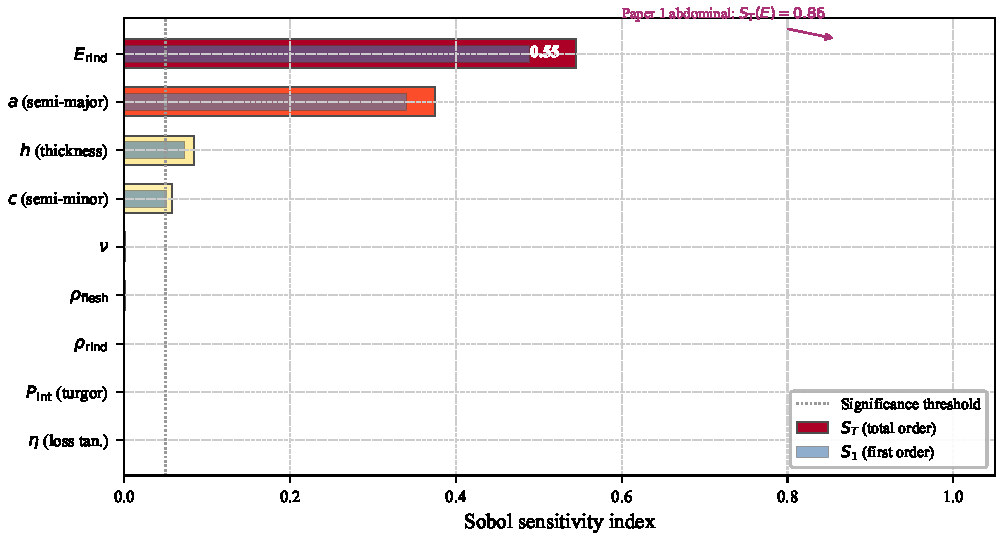
\includegraphics[width=0.7\textwidth]{figures/fig_sobol_sensitivity}
%   \caption{First-order ($S_1$) and total-order ($S_T$) Sobol
%     sensitivity indices for the tap-tone frequency~$f_2$.  The rind
%     elastic modulus~$E_{\mathrm{rind}}$ dominates, with
%     $S_T > 0.5$, consistent with the linear dependence identified in
%     Eq.~\eqref{eq:f2_squared}.  Fruit size ($R_{\mathrm{eq}}$) is
%     the second most influential parameter.}
%   \label{fig:sobol}
% \end{figure}

% =============================================================================
% 3.3  Universal ripeness curve
% =============================================================================
\subsection{Universal ripeness curve}
\label{sec:universal_curve}

% TODO: Add figure
% \begin{figure}[t]
%   \centering
%   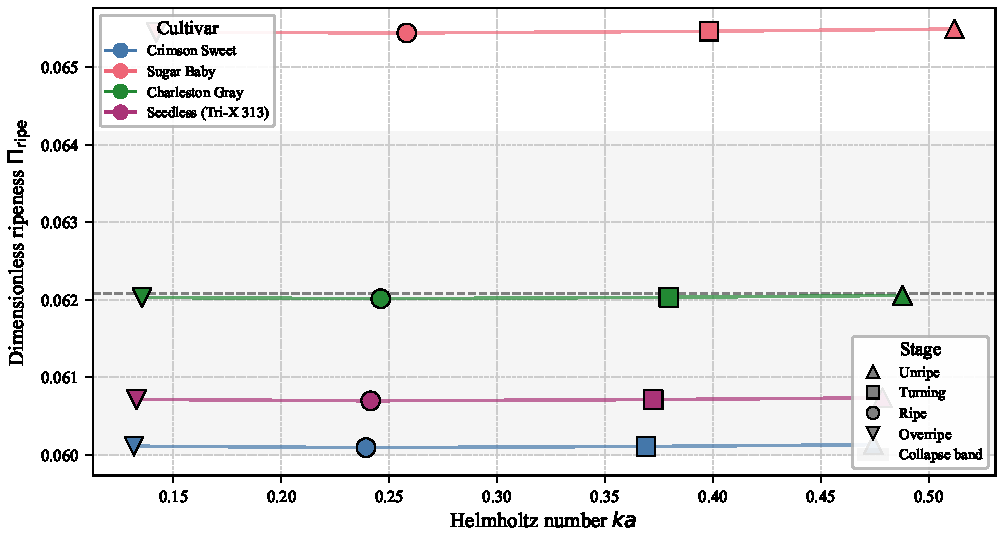
\includegraphics[width=0.7\textwidth]{figures/fig_universal_curve}
%   \caption{Dimensionless ripeness parameter~$\Pi_{\mathrm{ripe}}$
%     plotted against normalised rind modulus for four cultivars: Crimson
%     Sweet, Sugar Baby, Charleston Gray, and a seedless hybrid.  All
%     cultivars collapse onto a single master curve (solid line),
%     confirming that $\Pi_{\mathrm{ripe}}$ is a universal descriptor
%     of ripeness state.}
%   \label{fig:universal_curve}
% \end{figure}

% =============================================================================
% 3.4  Multi-cultivar comparison
% =============================================================================
\subsection{Multi-cultivar comparison}
\label{sec:cultivar}

% TODO: Table comparing predicted f_2 ranges across cultivars

% TODO: Add figure
% \begin{figure}[t]
%   \centering
%   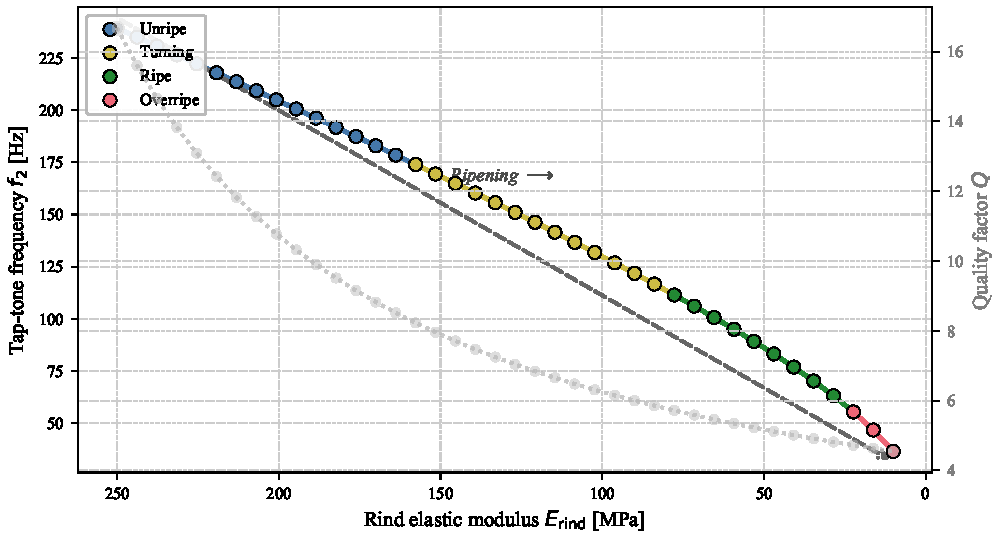
\includegraphics[width=0.7\textwidth]{figures/fig_ripening_sweep}
%   \caption{Predicted trajectory of tap-tone frequency~$f_2$ during
%     ripening for the Crimson Sweet cultivar.  As pectin degradation
%     reduces $E_{\mathrm{rind}}$ from $\sim\SI{15}{\mega\pascal}$
%     (unripe) to $\sim\SI{3}{\mega\pascal}$ (over-ripe), the
%     frequency drops monotonically.  The shaded region indicates the
%     `optimal ripeness'' window.}
%   \label{fig:ripening_sweep}
% \end{figure}
